\chapter{Pismo Wind Study (working title)}
% Replace with your specific project title

\section{Abstract}
% Brief summary of your research (250-300 words)
% Include: research question, methods, key findings, and conclusions

\section{Introduction}
% Background on monarch butterflies
% Research context and significance
% Specific research questions/hypotheses
\lipsum[1]  % Replace with your actual introduction text

\section{Materials and Methods}
% Detailed methods subsections
\subsection{Study Site}
% Description of where you conducted your research

\subsection{Experimental Design}
% Details of your experimental setup

\begin{figure}[htbp]
    \centering
    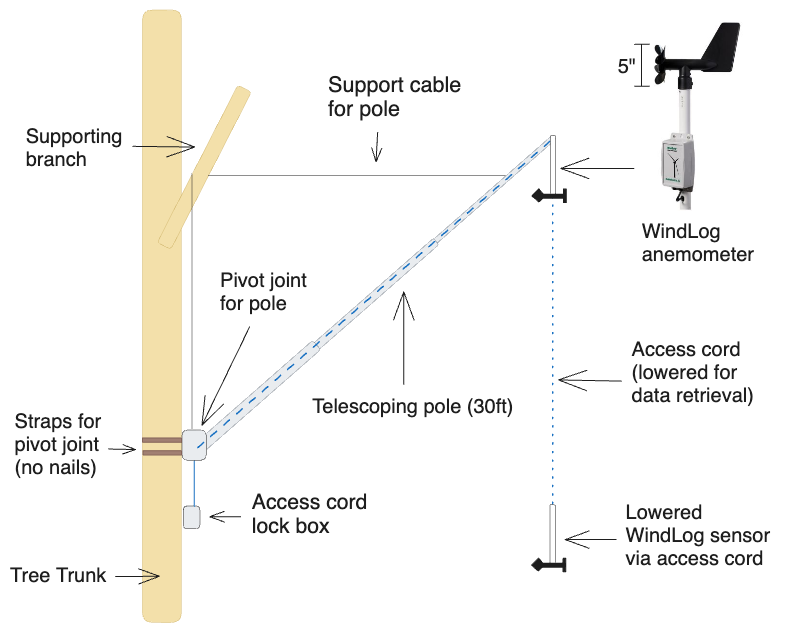
\includegraphics[width=3.5in]{figures/pismoPoleDiagram.png}
    \caption{Conceptual diagram of wind meter mounting apparatus}
\end{figure}




\subsection{Data Collection}
% How you gathered your data

\subsection{Statistical Analysis}
% How you analyzed your results

\section{Results}
% Present your findings
\lipsum[2]  % Replace with your actual results text


% Example of how to include a figure with caption
\begin{figure}[htbp]
    \centering
    \includegraphics[width=3.5in]{example-image}
    \caption{Clear, descriptive caption explaining what the figure shows and its significance.}
\end{figure}

\section{Discussion}
% Interpret your results
% Connect to broader context
% Address limitations
% Suggest future directions
\lipsum[3]  % Replace with your actual discussion text

\section{References}
% Your cited references will go here
% Format according to your target journal's style
